\documentclass{article}
\usepackage[a4paper, tmargin=1in, bmargin=1in]{geometry}
\usepackage[utf8]{inputenc}
\usepackage{graphicx}
\usepackage[justification=centering]{caption}

% \usepackage{parskip}
\usepackage{pdflscape}
\usepackage{listings}
\usepackage{hyperref}
\usepackage{caption}
\usepackage{subcaption}
\usepackage{float}
\usepackage{amsmath}
\DeclareMathOperator*{\argmax}{\arg\!\max}
\title{CS 747 : Foundations of Intelligent Learning Agents Assignment 2}
\author{Arka Sadhu - 140070011}
\date{\today}

\begin{document}
\maketitle

\section{Linear Programming}
The MDP problem is formulated as a linear programming problem. In total there are n variables and nk constraints where n is number of states and k is the number of actions.
\subsection{Objective}
The objective function is
$$\min \sum_{i=1}^n v_i$$
Here $v_i$ is the optimal value function for each state $i$. These are the n variables
\subsection{Constraints}
The constraints for the optimal value function is that for all $s \in S$ and $a \in A$, where $S$ is the set of all states, and $A$ is the set of all actions, we have:
$$v_s \ge \sum_{s'\in S}T(s, a, s')[R(s, a, s') + \gamma v_{s'}]$$
Here $T(s,a,s')$ is the transition matrix which gives the probability of transitioning from state s to s' when performing action a. $R(s,a,s')$ is the reward matrix which gives the reward on going from state s to s' on performing action a. $\gamma$ is a discount factor.

Since the constraint is for all $s \in S$ and for all $a \in A$ there are in total nk constraints.

The objective function, constraints and variables are passed on to PuLP which gives us the optimal value function $V^*(s)$

\subsection{Value function to Policy}
To get back the best policy we define a function
$$Q^*(s, a) = \sum_{s' \in S}T(s, a, s')[R(s,a,s') + \gamma V^*(s')]$$
And then get the optimal policy $\pi^*(s)$ as
$$\pi^* (s) = \argmax_{a \in A} Q^*(s,a)$$

\section{MDP Creation}
To create an MDP the following was used
\begin{itemize}
\item Set total number of states(S) to 50 and total number of actions(A) to 2.
\item Create a random reward matrix of size $S x A x S$ with each element in the range $[-1, 1]$.
\item Then create a random transition matrix of size $S x A x S$ with each element in the range $[0,1]$. We note that each eleement of the transition matrix $[s, a, s']$ gives the probability of transition from state $s$ to $s'$ on performing action $a$. Therefore we would need the sum of elements of the transition matrix from state $s$ and performing action $a$ to be 1. That is the agent can only go to one of the $s'$ states with a finite probability.
\item A discount factor $\gamma$ is created using a random number generator from $[0,1)$.
\end{itemize}

\section{Comparison between differe Policy Iteration}
\begin{figure}[H]
  \centering
  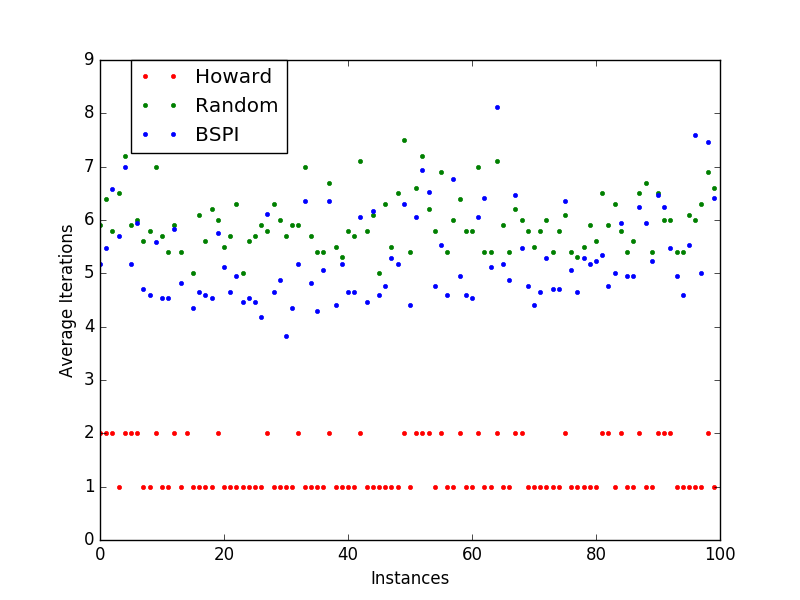
\includegraphics[scale=0.5]{images/Policy_Iteration_Plot}
  \caption{Plot of different Policy Iterations}
  \label{fig:1}
\end{figure}

The plot in \ref{fig:1} is generated in the following manner:
\begin{itemize}
\item For Howard PI, directly the number of iterations is plotted.
\item For Random PI, random seeds 0-9 are used, and the number of iterations for each of them is noted and then their mean is taken.
\item For Batch switch PI, batch sizes in step sizes of 3 were chosen in the range [1, 50] and the number of iterations for each is again noted and their mean is taken.
\end{itemize}
\section{Howard Policy Iteration}
For a total of 100 MDP instances with 50 states and 2 action policies.
\begin{table}[H]
\centering
\caption{Howard PI}
\label{t:hpi}
\begin{tabular}{|l|l|}
\hline
              & Howard PI \\ \hline
Mean          & 1.33      \\ \hline
Std deviation & 0.47021   \\ \hline
\end{tabular}
\end{table}

\section{Random Policy Iteration}
For a total of 100 MDP instances with 50 states and 2 action policies.
\begin{table}[H]
\centering
\caption{Random PI}
\label{t:rpi}
\begin{tabular}{|l|l|}
\hline
              & Random PI \\ \hline
Mean          & 5.977     \\ \hline
Std deviation & 0.5522    \\ \hline
\end{tabular}
\end{table}

For random seed [0-9]
\begin{table}[H]
\centering
\caption{Random PI with seeds}
\label{t:rpi_seeds}
\begin{tabular}{|l|l|l|}
\hline
Random Seed & Mean & Std dev        \\ \hline
0           & 5.35 & 0.841130192063 \\ \hline
1           & 6.04 & 1.29553077926  \\ \hline
2           & 5.72 & 1.96509541753  \\ \hline
3           & 4.63 & 1.04551422755  \\ \hline
4           & 7.39 & 1.57413468293  \\ \hline
5           & 6.66 & 1.97595546509  \\ \hline
6           & 6.8  & 1.75499287748  \\ \hline
7           & 5.13 & 0.976268405716 \\ \hline
8           & 5.89 & 1.52901929353  \\ \hline
9           & 6.16 & 1.32453765518  \\ \hline
\end{tabular}
\end{table}

\section{Batch Switching Policy Iteration}
For a total of 100 MDP instances with 50 states and 2 action policies.
\begin{table}[H]
\centering
\caption{Batch Switch PI}
\label{t:bspi}
\begin{tabular}{|l|l|}
\hline
        & Batch Switch PI \\ \hline
Mean    & 5.32764         \\ \hline
Std dev & 0.86229         \\ \hline
\end{tabular}
\end{table}

For batches in steps of 3 in the range of [1,50]
\begin{table}[H]
\centering
\caption{My caption}
\label{t:bspi_batches}
\begin{tabular}{|l|l|l|}
\hline
Batch Size & Mean  & Std Dev        \\ \hline
1          & 26.43 & 4.21011876317  \\ \hline
4          & 13.0  & 1.8973665961   \\ \hline
7          & 8.23  & 1.44813673388  \\ \hline
10         & 5.71  & 1.11619890701  \\ \hline
13         & 4.68  & 1.00876161703  \\ \hline
16         & 4.3   & 1.15325625947  \\ \hline
19         & 3.55  & 0.93139680051  \\ \hline
22         & 3.46  & 0.89911067172  \\ \hline
25         & 2.53  & 0.830120473184 \\ \hline
28         & 2.51  & 0.780960946527 \\ \hline
31         & 2.43  & 0.681982404465 \\ \hline
34         & 2.46  & 0.713021738799 \\ \hline
37         & 2.45  & 0.698212002188 \\ \hline
40         & 2.42  & 0.602992537267 \\ \hline
43         & 2.41  & 0.649538297562 \\ \hline
46         & 2.22  & 0.656962708226 \\ \hline
49         & 1.78  & 0.742697785105 \\ \hline
\end{tabular}
\end{table}

\section{Interesting Observations}
\begin{itemize}
\item Howard PI didn't take more than 2 iterations on any of the 50 state 2 action MDP. This is quite remarkable since the number of possible policies is $2^{50}$ and yet it is able to converge extremely fast. This is interesting because the worst case bound of Howard PI is $O(\frac{2^n}{n})$ and it is greater than both of Random PI and Batch Switch PI.
\item The possible explanation for Howard PI performing significantly better than random PI and Batch Switch PI is that Howard PI is a greedy algorithm, and for a 2-action MDP no two policies can have the same set of improvable set. Another possibility is that the Howard PI has a much tighter bound than the other two PI methods.
\item Random PI and Batch Switch PI both took on an average 5-7 iterations. Interestingly random PI was affected by the random seed quite significantly in a few cases. And in general random PI had a larger std deviation compared to the other two PI.
\item Batch Switch PI performs quite bad when the batch sizes are very small. It does much better when batch sizes become larger and the effect on number of iteration seems to be monotonic empirically. When the batch size is the same as
\end{itemize}

\section{Libraries Used}
All algorithms have been coded in Python3. Numpy is used for all matrix operations and sorting methods. PuLP is used for solving linear programming problem and also to get value function for a given policy. Matplotlib is used for generating the plots.

Numpy3 is not installed in the sl2 machines, and a bug has been filed in the cse bug tracking system.

\end{document}
